\documentclass[conference]{IEEEtran}
\IEEEoverridecommandlockouts
% The preceding line is only needed to identify funding in the first footnote. If that is unneeded, please comment it out.
\usepackage{cite}
\usepackage{amsmath,amssymb,amsfonts}
\usepackage{algorithmic}
\usepackage{graphicx}
\usepackage{textcomp}
\usepackage{xcolor}
 \usepackage{multirow}
 \usepackage[utf8]{inputenc}
 \usepackage[T1]{fontenc}

%---------------------------------
%By Ti
%% Кодировки и шрифты %%%
%\usepackage{cmap}						% Улучшенный поиск русских слов в полученном pdf-файле
%\usepackage[utf8]{inputenc}				% Кодировка utf8
%\usepackage[english, russian]{babel}    % Языки: русский, английский
%\usepackage[T2A]{fontenc}				% Поддержка русских букв
%\usepackage{pscyr}
%\usepackage{booktabs}						% Красивые русские шрифты
%---------------------------------

\def\BibTeX{{\rm B\kern-.05em{\sc i\kern-.025em b}\kern-.08em
    T\kern-.1667em\lower.7ex\hbox{E}\kern-.125emX}}

\def\BibTeX{{\rm B\kern-.05em{\sc i\kern-.025em b}\kern-.08em
T\kern-.1667em\lower.7ex\hbox{E}\kern-.125emX}}

\begin{document}

\title{Comparison of Elliptical and Spherical Geometric Model of the Heart for Computer Multichannel Electrical Impedance Cardiography\\
%{\footnotesize \textsuperscript{*}Note: Sub-titles are not captured in Xplore and
%should not be used}
\thanks{The reported study was funded by RFBR according to the research project No 18-29-02042.}
}

\author{\IEEEauthorblockN{Alexey Tikhomirov}
\IEEEauthorblockA{\textit{Bauman Moscow State Technical} \\
\textit{University}\\
Moscow, Russia \\
tikhomirov.an@bmstu.ru}
\and
\IEEEauthorblockN{Andrey Briko}
\IEEEauthorblockA{\textit{Bauman Moscow State Technical} \\
\textit{University}\\
Moscow, Russia \\
briko@bmstu.ru}
\and
    \IEEEauthorblockN{Nikolay Seleznev}
\IEEEauthorblockA{\textit{Bauman Moscow State Technical} \\
\textit{University}\\
Moscow, Russia \\
seleznev.nv@bk.ru}
\and
\IEEEauthorblockN{\ }
\IEEEauthorblockA{\ }
\and
\IEEEauthorblockN{Arman Petrosyants}
\IEEEauthorblockA{\textit{Bauman Moscow State Technical} \\
\textit{University}\\
Moscow, Russia \\
petrosyantsaa@student.bmstu.ru}
\and

\IEEEauthorblockN{\ \ \ \ \ \ \ \ \ \ \ \newline}
\IEEEauthorblockA{\ \ \ \ \ \ \ \ \ \ \ \\
\ \ \ \ \ \ \ \ \ \ \ \ \ \ \ \ \ \ \ \ \ \ \ \ \ \ \ \ \ \ \ \ \ \ \ \ \ \ \ \ \ \ \ \ \ \ \ \ \ \ \ \ \ \ \ }
\and
\IEEEauthorblockN{Sergey Shchukin}
\IEEEauthorblockA{\textit{Bauman Moscow State Technical} \\
\textit{University}\\
Moscow, Russia \\
0000-0002-9890-5267}
%\and
%\IEEEauthorblockN{6\textsuperscript{th} Sergey Shchukin}
%\IEEEauthorblockA{\textit{Bauman Moscow State Technical} \\
%\textit{University}\\
%City, Country \\
%email address or ORCID}
}
\IEEEaftertitletext{\vspace{-2\baselineskip}}
\maketitle

\begin{abstract}

    Development of electrical impedance methods for examining heart goes in three directions.
    These directions are transthoracic rheocardiography, electrical impedance tomography (EIT), and precordial rheocardiography.
    This bifurcation is due to the need for medicines used in the non-invasive methods that allow monitoring heart’s activity hemodynamic characteristics.
    This work focuses on the methods of precordial rheocardiography.
    This research takes into consideration the geometric models which are used to solve the inverse problem of impedance measurement in precordial rheocardiography.
    The various geometrical models of heart blood (3D model, sphere model and ellipsoid model) which are obtained by approximating the original 3D model, have been compared.
    The comparison has been done for volumetric characteristics and displacements of the mass model center during the cardiac cycle.
    The studies have shown that for a given volunteer, an elliptical geometric model of heart blood approximates the heart real 3D geometry with error of 3-5\%.
    This elliptical geometric model is preferable when assessing hemodynamic parameters.
    Based on electrical impedance modeling results, it has been concluded that for small electrode systems typical of precordial radial mapping, the ellipse model is preferable.
    For longitudinal-transverse mapping with large electrode systems, the sphere model is preferable.

\end{abstract}

\begin{IEEEkeywords}
    Impedance cardiography, 3D model heart, approximation, electrical impedance computer cardiography, sphere, ellipsoid
\end{IEEEkeywords}

\section{Introduction}

Stroke volume (SV), cardiac output (CO), and ejection fraction (EF) are crucial parameters for cardiovascular system assessment.
These parameters highlight the circulatory dynamics of the heart.

Circulatory parameters in clinical research and practice are assessed with CT, MRI, and ultrasound.
These methods provide loads of valuable diagnostic information on the heart.
However, continuous monitoring with these methods is not possible due to financial and dosimetric reasons.

Thermal dilution through pulmonary artery catheterization (PAC) is a golden standard of SV determination.
However, a set of non-invasive or minimally invasive procedures are extensively used ~\cite{Kobe2019},\cite{Mehta2014}.

LiDCO uses the minimally invasive method which is lithium chloride dilution ~\cite{Linton1993} .
Despite its minimal invasiveness, this method has a drawback.
The system should be calibrated when the hemodynamic condition changes or every 8 hours.
Moreover, one of the counter-indications of LiCl dilution is its intolerance to lithium.
PiCCO and FloTrac use contour analysis of pressure curve ~\cite{Horster2012}, which is accessed invasively via catheter.
Valve regurgitation, severe arrhythmia, and rapid changes in body temperature may affect measurements accuracy.

Electrical impedance methods of CVS study are non-invasive and inexpensive.
Among these methods are transthoracic methods, electrical impedance tomography, and precardial impedance cardiac plethysmography.

Transthoracic electrical impedance plethysmography (TEIP) traces back to the middle of the XX century.
It is currently used with minor changes in such apparatus as CardioScreen (Medis) and Rheo-Spectre (Neurosoft).
Non-invasive methods have few complications when used, but they are not free of drawbacks.
TEIP method is used to estimate changes and trends when assessing blood parameters.
However, it is not used in determining the absolute values.

Impedance cardiography (ICG) applies to both lungs and heart studies~\cite{Brown2003, Wu2018}.
The main disadvantage of using ICG is low spatial resolution in terms of assessing heart hemodynamics problem~\cite{Kircher2019, Rymarczyk2019}.

In 2002, a precardial mapping technique was proposed to expand electrical impedance methods for heart studies.

\section{Materials and methods}

\subsection{Precardial Impedance Cardiography Methods}

The precardial impedance cardiography combines several methods.
Precardial radial mapping method is the first method.
The electrode systems are located along the ventricle projection border onto the chest surface perpendicular to the border~\cite{Timokhin2014},\cite{Tikhomirov2019}.
The second method is longitudinal-transverse mapping.
In this method, one electrode system is located on the chest’s surface above the heart along the heart’s anatomical axis and the other is perpendicular to the axis.

Precardial impedance cardiography is based on the inverse problem of the electrical impedance measurements.
The geometric model is built depending on the priori anatomical data which are generally provided via the CT or MRI.
Heart is modeled as a sphere, ellipsoid, or more complex geometry.
Heart contraction is represented by changing the parameters of the model such as the sphere radius.
The experimentally recorded changes in electrical impedance during heart contraction are converted into changes in the geometric model parameters based on the solution of the inverse problem.
After that, the volumetric characteristics are estimated.

Complexity of chest and heart geometric models imposes a larger number of parameters that describe heart contraction in more details.
However, this situation requires a larger number of electrode systems to obtain data for solving the inverse problem of electrical impedance measurement.

Hence, a more complex model allows obtaining more information and requires more electrode systems.
A simpler model requires fewer electrode systems.
However, this model is limited in capabilities.
It is necessary to find a compromise between the model complexity and the output information of the model.

In circulatory characteristics monitoring, vanity and simplicity of the technique are often more critical.
This research compares two geometric models of a homogeneous half-space with a sphere and ellipsoid inclusions.
Both the models are considered for the method of precordial longitudinal-transverse cardiac mapping.

\subsection{Ellipsoid and Sphere models}

In simulation, heart blood is often represented as the sphere in electrical impedance measurement problems, in precordial mapping methods~\cite{Tikhomirov2019}, and in electrical impedance tomography of the heart.

This model is quite simple.
According to the tomography data, sphere’s parameters the radius and coordinates of the center are determined.
Heart contraction corresponds to a change in the sphere radius and offset of its center.

The ellipsoid model allows a better approximation of blood in the heart before the onset of ventricular systole.
% статьи по эллипсу

However, number of model parameters (three semiaxes of the ellipsoid, coordinates of the center, and rotation of the ellipsoid in space) increases compared to one radius and center’s coordinates.
Heart contraction corresponds to a change in the semiaxes of the ellipsoid and a shift in its center.
The ellipsoid can also be spatially rotated during contraction.

Models’ geometric parameters were obtained from CT data of a healthy volunteer.
The study of multi-spiral computed tomography was carried out in Pirogov Moscow City Clinical Hospital using Toshiba Aquilion PRIME 160.
%It was done under patronage of employees of both the clinic and the medical center of the BMSTU medical center.

The study was carried out by introducing an iodine-containing contrast
agent Optiray 350 mg, 90 ml for the study on inspiration and 90 ml for the study
on exhalation, 50 ml at a rate of 3.5 ml/sec, and 40 ml at a rate of 3 ml/sec.

The study was carried out on free expiration.
As a result of these studies’ reconstruction, sets of slices with a time resolution of 20 series per cardio cycle were obtained which give about 35-50 ms between the series.
Distance between the axial slices was 2.5 mm.
The sets of sections were used to reconstruct a 3D model of blood in the heart~\ref{fig:wall}.
%Использовалось программное обеспечение ИНОБИНЕК 2.2.1 Профессиональная редакция.
The software used was INOBITEK 2.2.1 Professional edition.

\subsection{Sphere and Ellipsoid Approximation}

Parameters of the sphere and ellipsoid were obtained by approximating 3D models of the heart’s blood.
The sphere was approximated by criterion of the least square deviation of the sphere boundaries and real 3D geometry.
Approximation criterion~\ref{eq:sphere_criteria},
$p_i$ - a finite set of points on the surface of a 3D heart model,
$dist(p_i,Z(f))$ -  distance from the point $p_i$ to the surface of the sphere $Z(f)$.
\begin{equation}
    \sum_{i=1}^{q}dist(p_i,Z(f))^2 \rightarrow min
    \label{eq:sphere_criteria}
\end{equation}

The ellipsoid was obtained according to the criterion described in~\cite{Bookstein1979}.
The method is peculiar because authors consider the distance from a point to the ellipsoid as follows.

Difference between the distance from the center of the ellipsoid to the point and the distance from the center of the ellipsoid to a point on its boundary.
The mentioned point lies on the ray outgoing their center and passing through a given point.
Error of this assumption is estimated depending on the ratio of the ellipsoid semiaxes and an adjustment is made accordingly.
The final optimization criterion is also the least square method~\ref{eq:sphere_criteria}.

Analysis of the results and visualization of the approximation showed that the heart septa, such as the inter-ventricular septum, and the atrioventricular septum
(Fig.~\ref{fig:wall})
forms points that distort the approximation results.
This in turn causes increase in the average deviation of the approximating ellipse's surface or the sphere from the outer boundary of the 3D blood model.
%----------------------------------------------------------------------------
\begin{figure}[tbph]
    \centering
    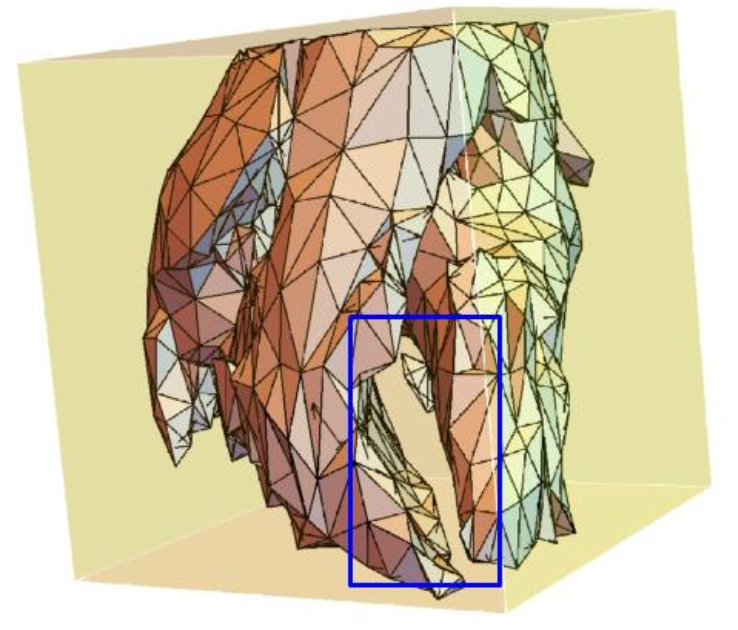
\includegraphics[width=0.55\linewidth]{fig/wall}
    \caption{3D model of blood in the heart (interventricular septum highlighted in blue)}
    \label{fig:wall}
\end{figure}
To eliminate this problem, it was decided to fill in the original 3D models of the heart partitions and internal voids.
For doing this, the 3D model was laid out on 2D images obtained by sectioning into planes parallel to the X and Y axes (Fig.~\ref{fig:algo}).
The distance between the planes is 1 mm.
%Расстояние между плоскостями 1 мм.

%--------------------------------------------------------
\begin{figure}[tbph]
    \centering
    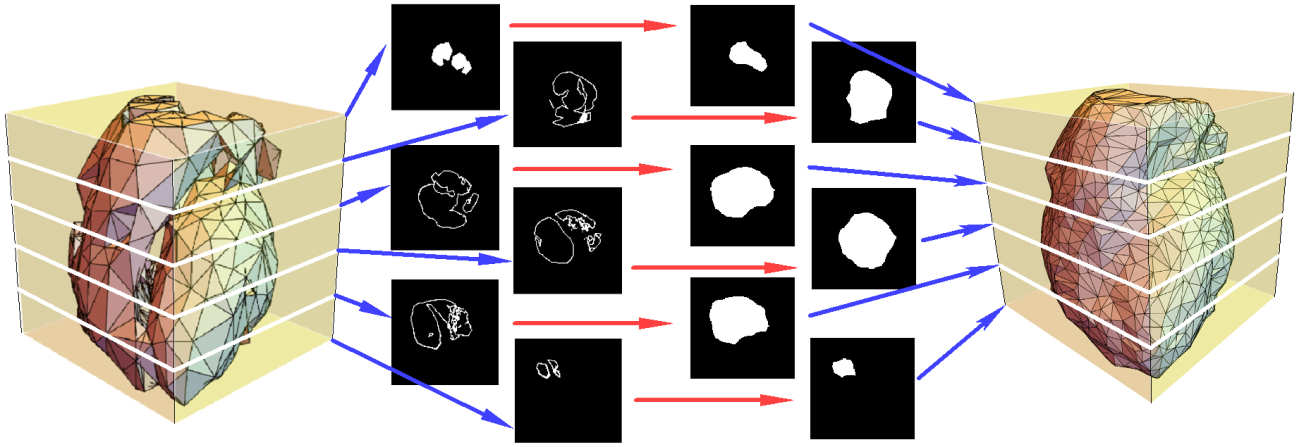
\includegraphics[width=\linewidth]{fig/algo}
    \caption{Algorithm for filling the septa of the heart in the 3D model of the heart's blood
    (on the left - the original 3D model, on the right - the 3D model after filling the septa)}
    \label{fig:algo}
\end{figure}
%---------------------------------------------------------

After that, a tangent path traversal was made of the 2D image contour with a circle radius of 20 mm (red circle)(Fig.~\ref{fig:algo2}), as a result of a set of obtained sections filled with septum was going to the 3D image of the heart.

%Затем 3D изображение преобразовывалось в STL модель с количеством граней 5000. Алгоритм реализован в Wolfram Mathematica на основе функции CLOSING.
Then the 3D image was converted into an STL model with 5000 faces.
The algorithm is implemented in Wolfram Mathematica based on the function - CLOSING.

\begin{figure}[tbph]
    \centering
    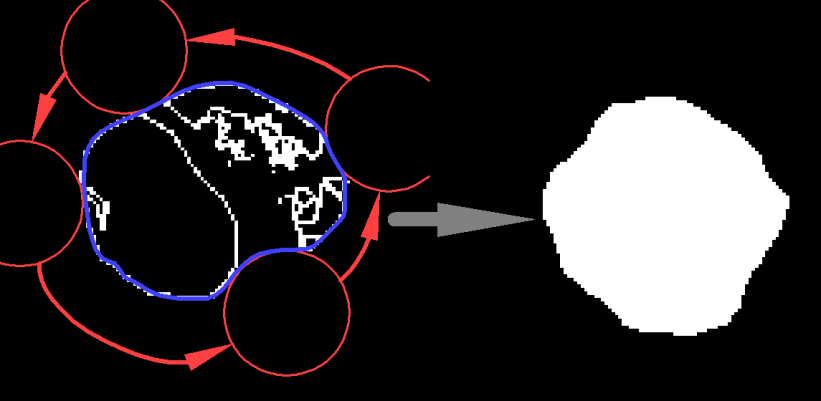
\includegraphics[width=0.9\linewidth]{fig/algo2}
    \caption{Tangent path traversal of a 2D image with a circleto fill heart's semptum
    in the 3D models of heart's blood (on the left is white contour beforethe septum filling,
        on the right side - after the filling)}
    \label{fig:algo2}
\end{figure}

\section{Modelling}
\subsection{Electrical Impedance modelling parameters}

To analyze the obtained geometric models, electrical impedance modeling has been carried out using the Comsol Multiphysics CAD.
Location of the electrode systems during modeling corresponds to location of the electrode systems during longitudinal-transverse mapping.
The distance between the current electrodes varied from 80 to 240 mm.
Ratio of distance between the current electrodes to the distance between the potential ones was 2 to 1.

Values of the resistivity of inclusion and homogeneous half-space are presented in table~\ref{tab:table}.

\begin{table}[htbp]
    \caption{Resisitivity values at  100 kHz used in the model study}
    \begin{center}
        \begin{tabular}{|l|c|c|}
            \hline
            \multirow{2}{*}{\textbf{Tissue}}              &     \textbf{Resistivity values,}      &    \textbf{Resistivity value in}  \\
            &   \textbf{$\Omega \cdot$ m}     &   \textbf{ simulation, $\Omega \cdot$ m} \\
            \hline
            Blood (Hct=50)           & 1.35\cite{Hill1975}           & 1.35      \\
            \hline
            Myocardium               & 4.6 \cite{Hasgall}       & \multirow{7}{*}{4.2}\\
            \cline{1-2}
            \multirow{2}{*}{Muscles} & 2.7 \cite{Hasgall}           &     \\
            \cline{2-2}
            & 1.5 – 25 \cite{Rush1963}           &   \\
            \cline{1-2}
            Lung (deflated)          & 3.68 \cite{Hasgall}     &         \\
            \cline{1-2}
            Lung                     & 1.6 - 10 \cite{Grimnes2008}       &    \\
            \cline{1-2}
            Human thorax & \multirow{2}{*}{4.63 \cite{Rush1963} }  &   \\
            (average)   & &   \\
            \hline
        \end{tabular}
        \label{tab:table}
    \end{center}
\end{table}
%todo поправить список литературы в таблице

%The averaging of the specific resistances of the lung, muscle tissue, and
%myocardium is possible since measurements are considered in the phase of calm
%expiration, and the specific resistance of the lung tissue on expiration
%approaches the specific resistance of muscle tissue.

Averaging of the specific resistances of lung, muscle tissue, and myocardium is possible since measurements are considered in the phase of calm expiration.
The specific resistance of lung tissue on expiration approaches the specific resistance of muscle tissue.

\subsection{Comparison of the 3D model with sphere and ellipsoid}

Several parameters were used for comparing the models themselves and the results of modeling the real 3D geometry of blood in heart, sphere, and ellipsoid.
A comparison of the change in the volume of blood in heart was made first.
Volume of a real 3D model was compared with the volumes of the approximating sphere and ellipsoid.
The volumes were estimated for each of the 20 points when the cardio cycle was split.
Second, movement of blood volume in heart as a whole was considered,
i.e. the movement of mass center of a real 3D model and its approximating figures.
Third, electrical impedance change dependencies during the cardiac cycle were compared for different positions and sizes of electrode systems.

\begin{figure}[htbp]
%    \centerline{
\includegraphics{fig/fig1.png}}
    \centering{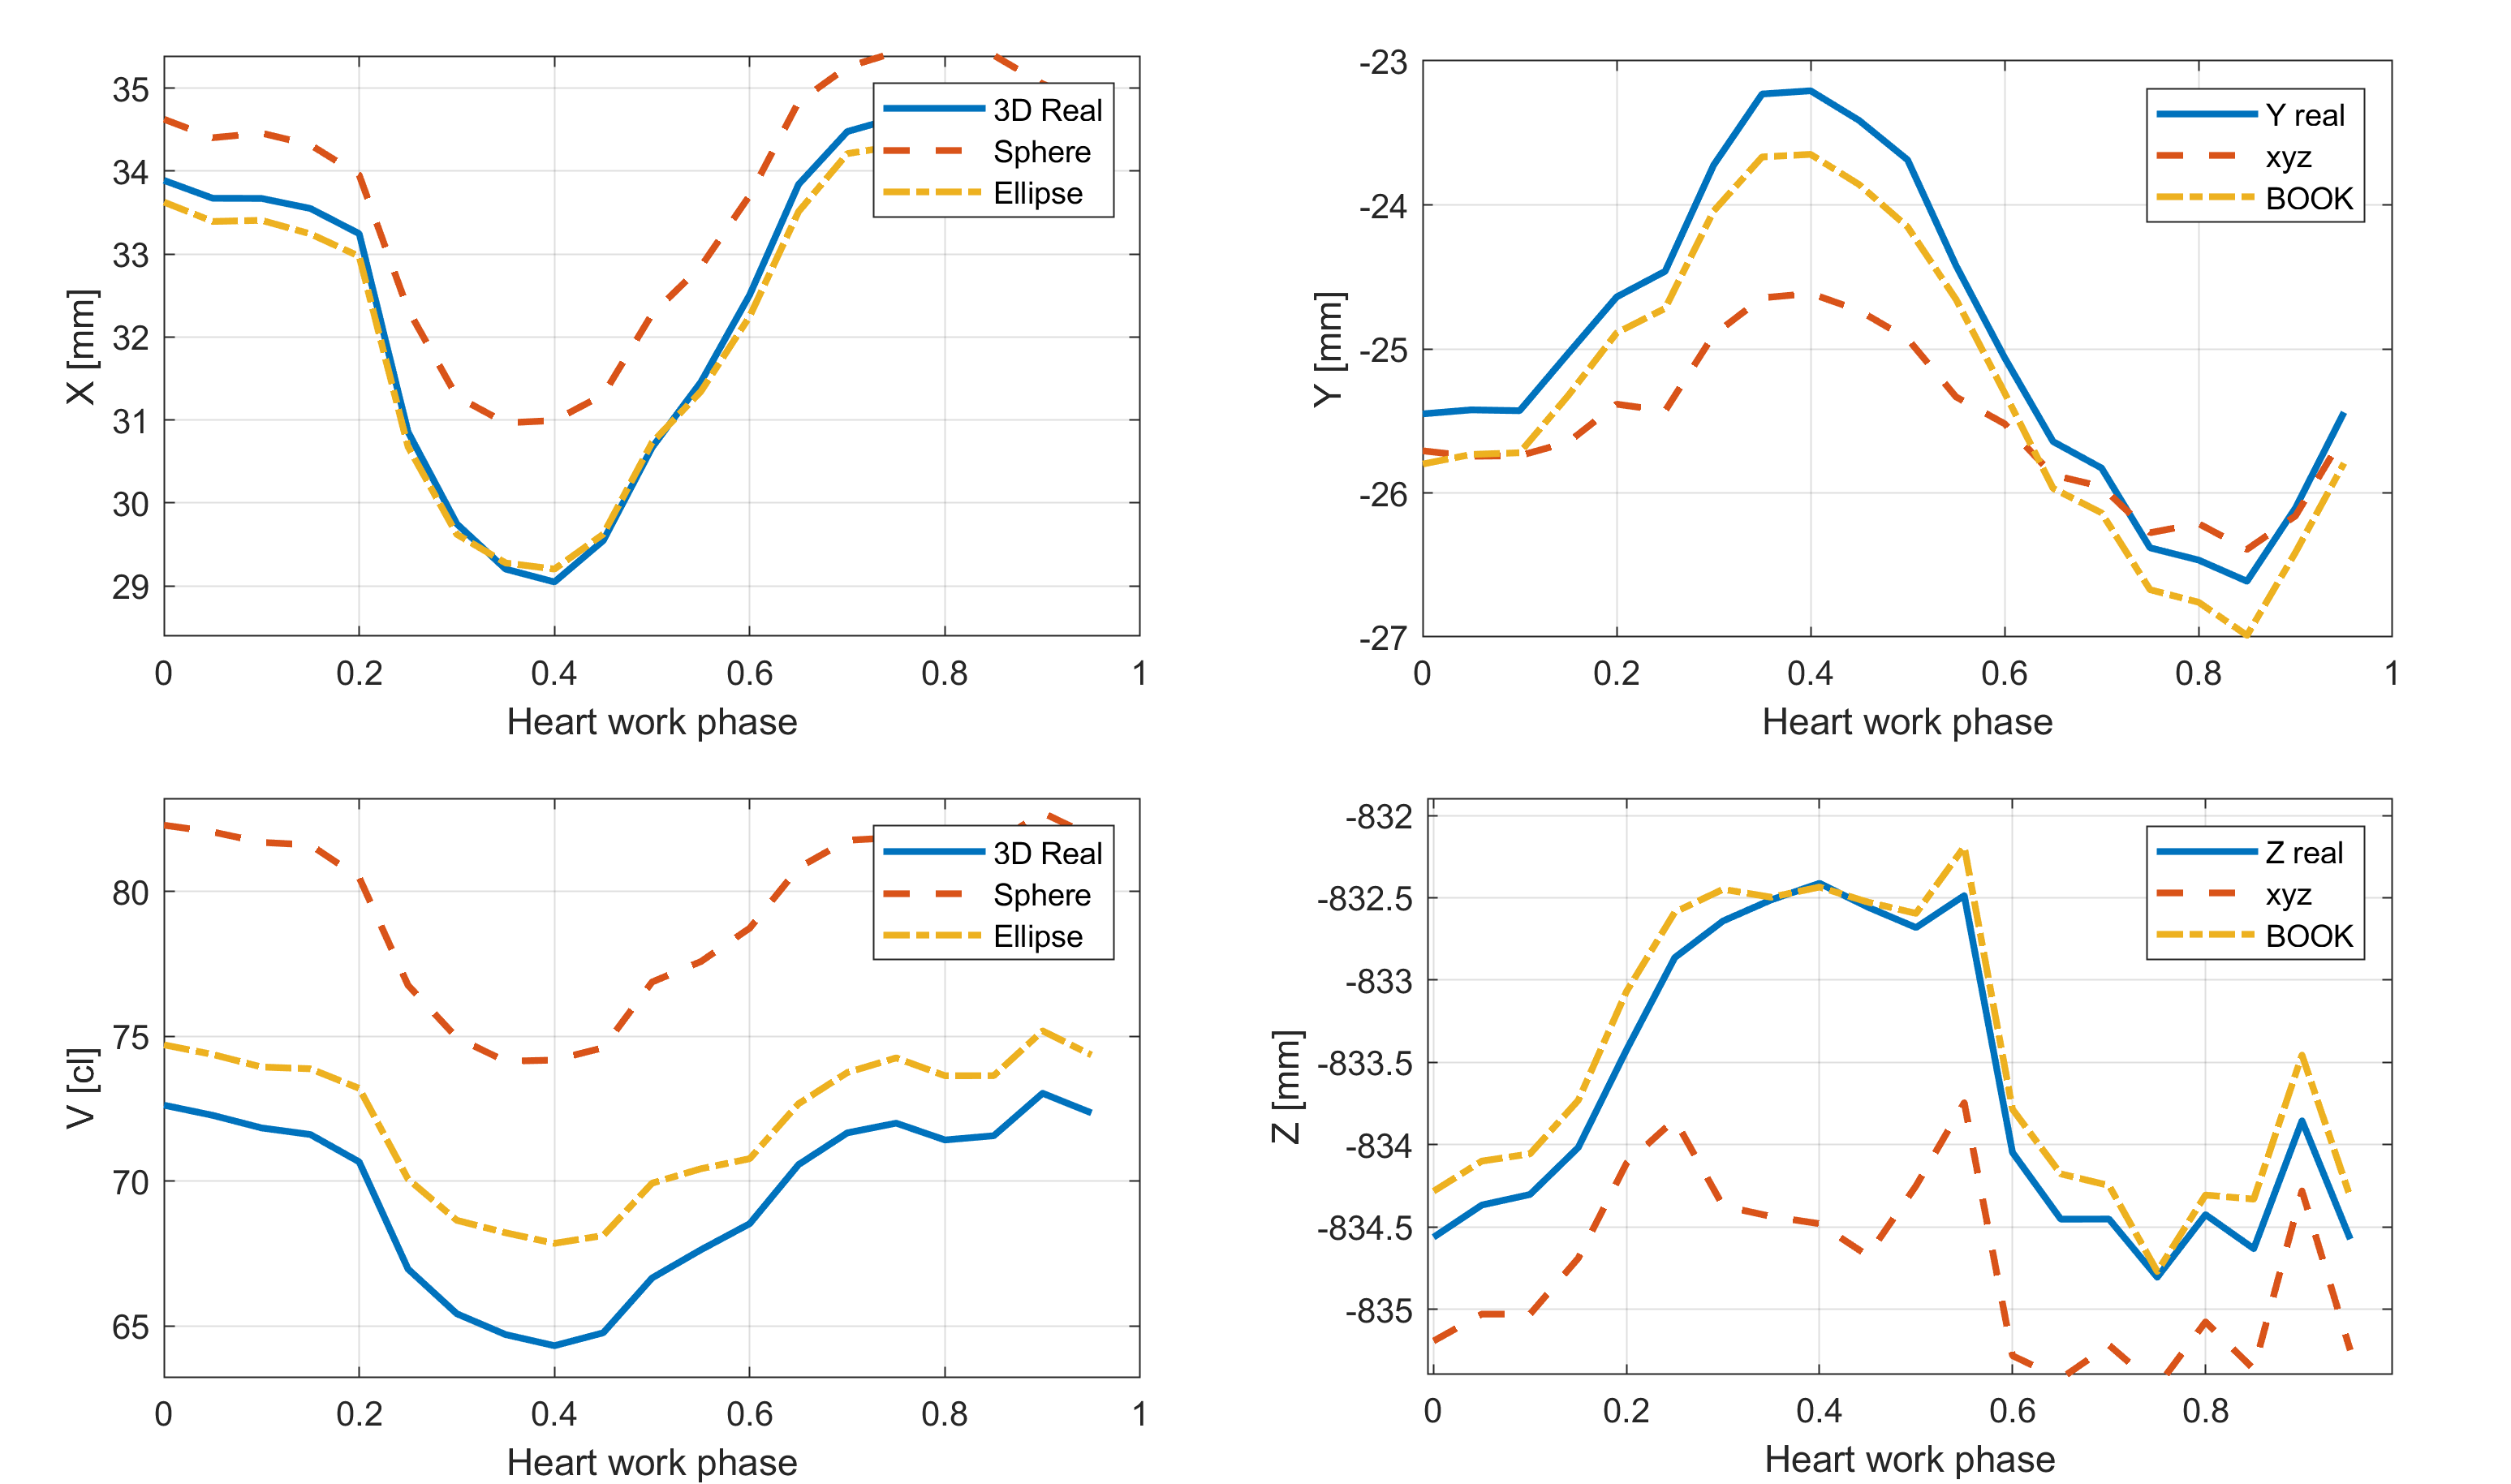
\includegraphics[width=\linewidth]{fig/1_4}}
    \caption{Change during the cardiac cycle of the coordinates of the center of mass (X, Y, Z) and volume of the original 3D model, sphere and ellipsoid}
    \label{fig:rxyz}
\end{figure}

\section{Results}

Dependences of the change in volume and mass center coordinates of the original 3D model, the sphere, and the ellipsoid are shown in
Fig.~\ref{fig:rxyz}.
Where the t-axis is R-to-R interval of cardiac cycle.
% по оси абсцисс

Simulation results of impedance changes during the cardiac cycle are presented in
%presented in Fig. ~\ref{real}, Fig.~\ref{fig:sphere}, Fig.~\ref{fig:ellipse}.
 Fig. ~\ref{fig:all}.
For each model, dependences are presented for the electrode system located along the heart anatomical axis and perpendicular to it.
These graphs also consider the cardiac cycle from R-wave to R-wave.

\begin{figure}[tbph]
    \centering
    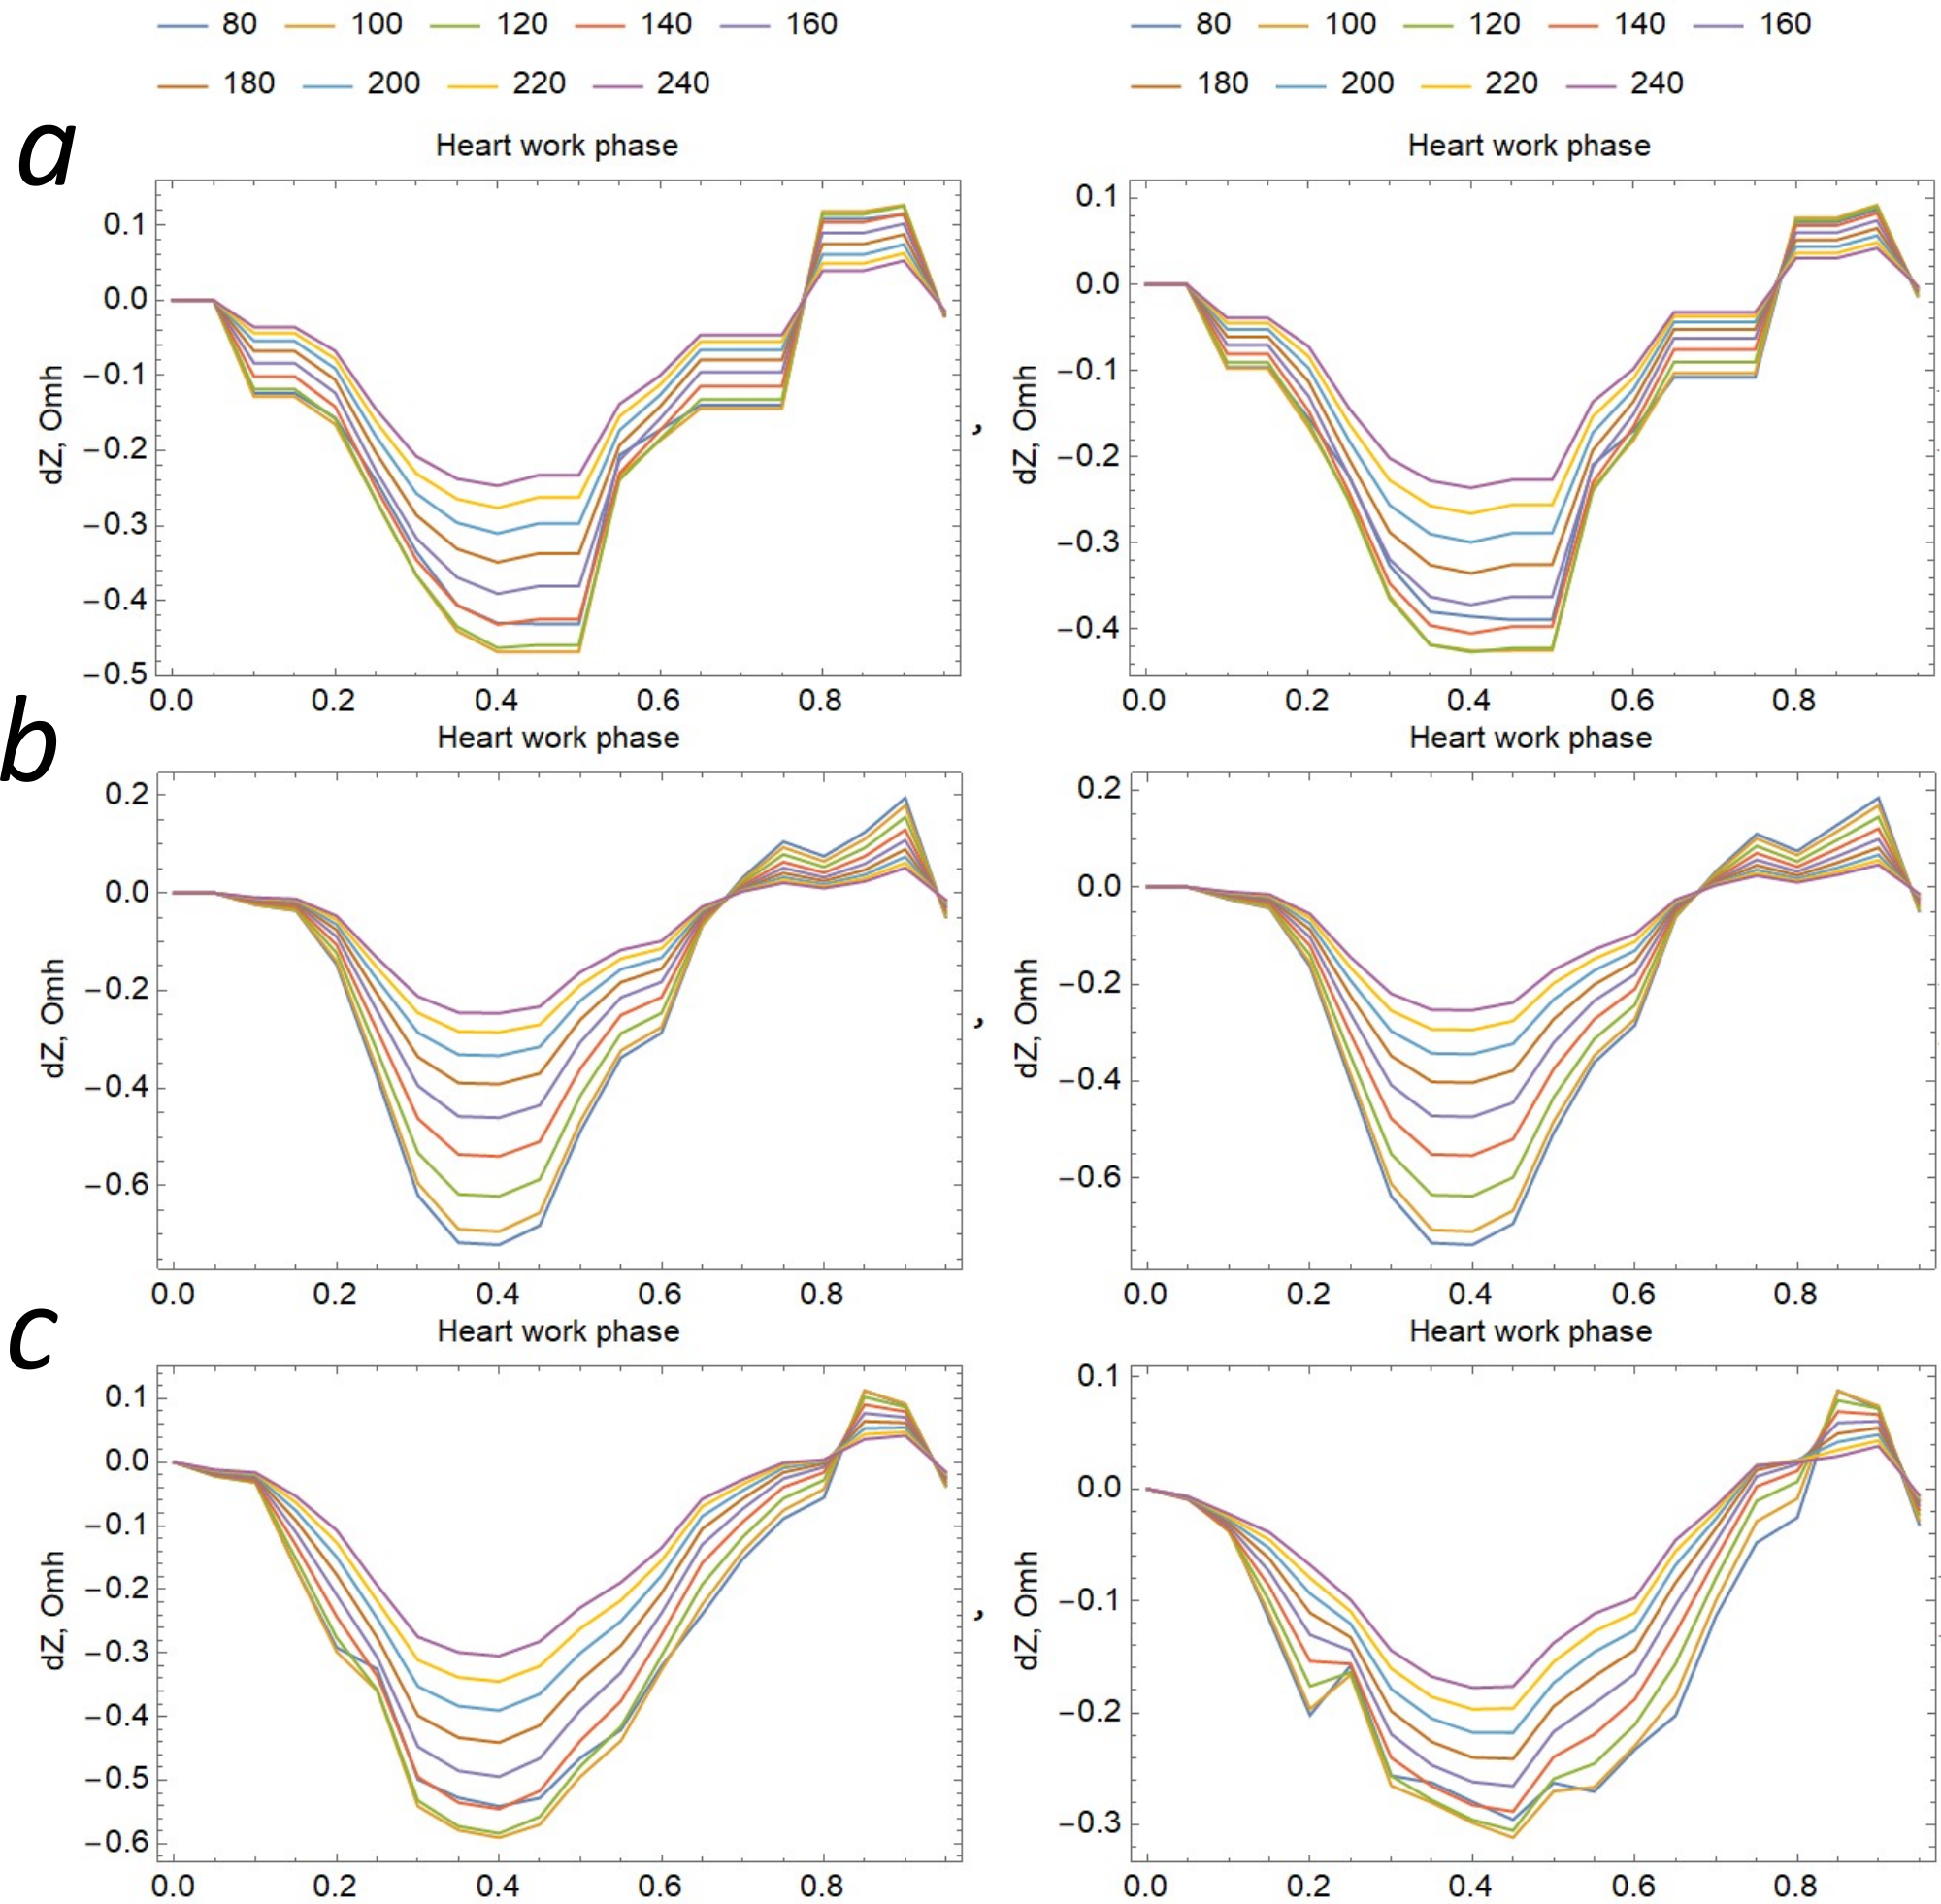
\includegraphics[width=\linewidth]{fig/all}
    \caption{Dependence of electrical impedance changes during the cardiac cycle for: a) initial 3D model b) spherical model c)elliptical model. Location of the electrode system along the heart axis - to the left, perpendicular to the heart axis - to the right.}
    \label{fig:all}
\end{figure}


%\begin{figure}[tbph]
%    \centering
%    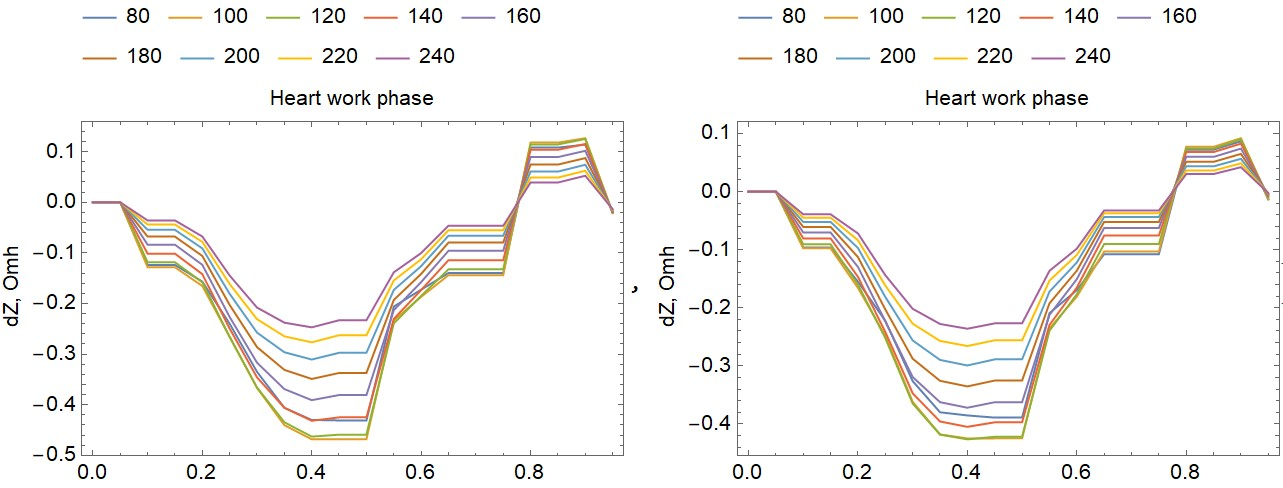
\includegraphics[width=\linewidth]{fig/real}
%    \caption{Dependence of electrical impedance changes during the cardiac cycle for the initial 3D model (location of the electrode system along the heart axis - to the left, perpendicular to the heart axis - to the right)}
%    \label{real}
%\end{figure}
%
%\begin{figure}[tbph]
%    \centering
%    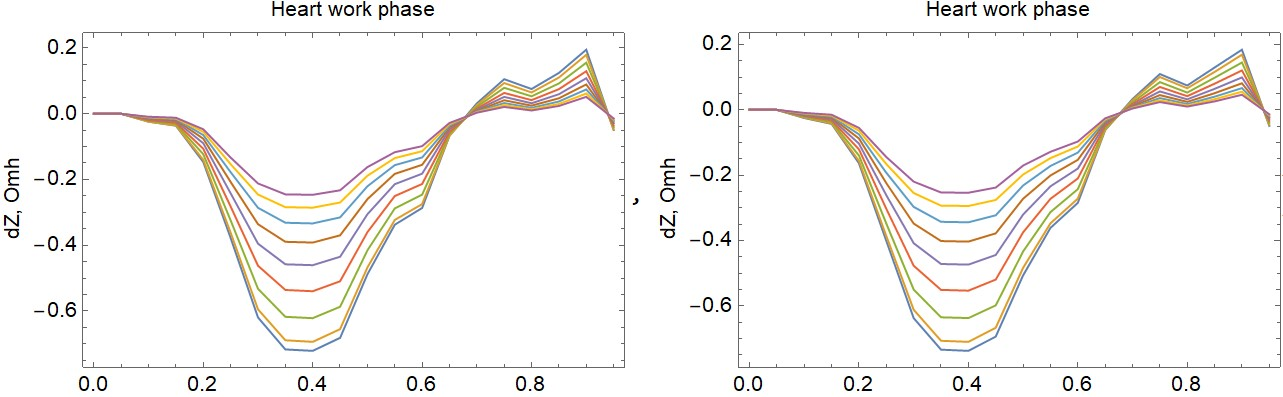
\includegraphics[width=\linewidth]{fig/sphere}
%    \caption{Dependence of electrical impedance changes during the cardiac cycle for a spherical model (the location of the electrode system along the heart axis - to the left, perpendicular to the heart axis - to the right)}
%    \label{fig:sphere}
%\end{figure}
%
%\begin{figure}[tbph]
%    \centering
%    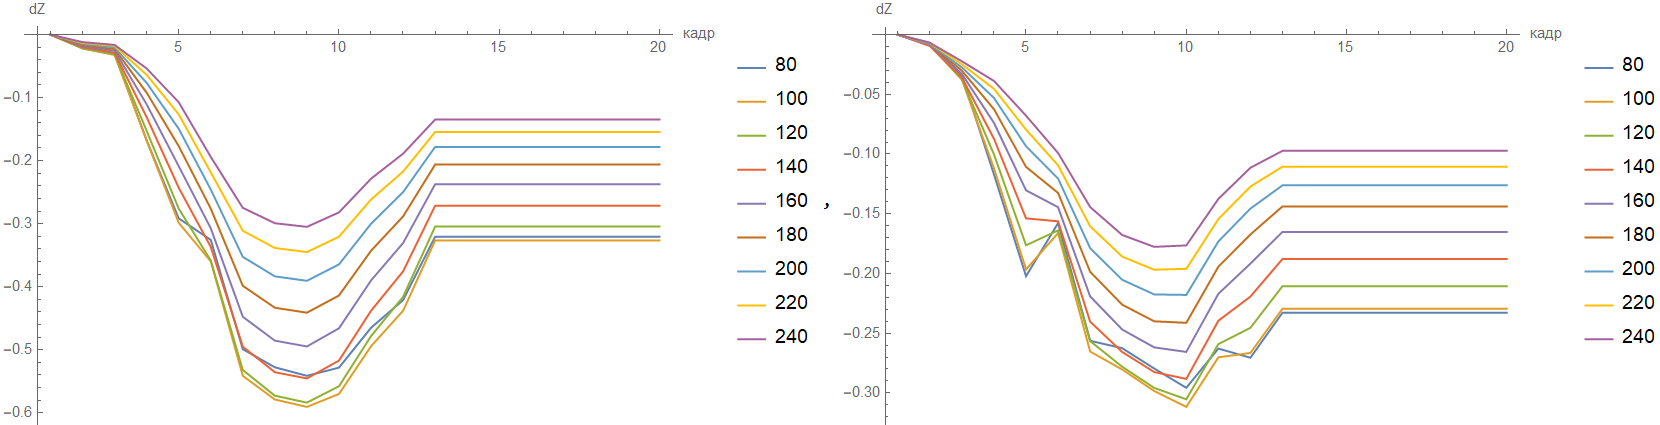
\includegraphics[width=\linewidth]{ellipse}
%    \caption{Dependence of electrical impedance changes during the cardiac cycle for an elliptical model (the location of the electrode system along the heart axis - on the left, perpendicular to the heart axis - on the right)}
%    \label{fig:ellipse}
%\end{figure}

\section{Discussion}

When comparing mass center motion of the original 3D model with the approximating sphere and ellipsoid from Fig.~\ref{fig:rxyz},
it is noticed that mass center of the ellipsoid moves in accordance with mass center of the 3D model.
The sphere movement qualitatively corresponds to the 3D model movement, but quantitatively it differs i.e. it has less amplitude.
The ellipsoid volume differs by an average of 3-5\% during the cardiac cycle.
The difference in case of the sphere reaches 12-15\%.
This effect can influence and introduce additional errors in assessing hemodynamic characteristics based on the sphere geometric model.
%The waveforms of the electrical impedance modeling signal for the sphere and the
%ellipsoid qualitatively correspond to the initial 3D model waveform but differ
%significantly in amplitude characteristics. For a numerical assessment of the
%obtained simulation results, the value of the impedance change during
%ventricular systole $ \Delta Z $ was compared. The difference in values in
%Fig.~\ref{fig:all}a at the time points corresponds to 0\% and 40\% of the cardiac
%cycle (beginning and end of ventricular systole). For small electrode systems
%(80-120 mm), $\Delta Z$ for a 3D model differs more then 50\% from $\Delta Z $ for a
%sphere and 25-30\% from $\Delta Z$ for an ellipsoid.
%For large electrode systems
%(200-240 mm), $\Delta Z$ for a 3D model differs by 5-10\% from $\Delta Z$ for a
%sphere and 30\% from $\Delta Z $ for an ellipsoid.%todo заполнить проценты


Waveforms of the electrical impedance modeling signal for the sphere and the ellipsoid qualitatively correspond to the initial 3D model waveform.
However, they differ significantly in amplitude characteristics.
For a numerical assessment of the obtained simulation results, value of the impedance change during ventricular systole $ \Delta Z $ was compared.
Difference in values in Fig.~\ref{fig:all}a at the time points corresponds to 0\% and 40\% of the cardiac cycle (beginning and end of ventricular systole).
For small electrode systems (80-120 mm), $\Delta Z$ for a 3D model differs more than 50\% from $\Delta Z$ for a sphere and 25-30\% from $\Delta Z$ for an ellipsoid.
For large electrode systems (200- 240 mm), $\Delta Z$ for a 3D model differs by 5-10\% from $\Delta Z$ for a sphere and 30\% from $\Delta Z$ for an ellipsoid.

\section{Conclusion}

The studies have shown that for a given volunteer, an elliptical geometric model of  heart blood approximates the heart real 3D geometry with error of 3-5\%.
This elliptical geometric model is preferable when assessing hemodynamic parameters.
Simultaneously, electrical impedance modeling showed that when using 80-120 mm in size electrode systems, it is preferable to use an elliptical geometric model.
On the other hand, when using large electrode systems (200-240 mm), it is preferable to use a spherical geometric model.
Since electrode systems with sizes over 180 mm are usually used for precordial longitudinal-transverse mapping, it is necessary to use a spherical mathematical model.

The drawn conclusions are valid for this volunteer.
At the moment, studies are underway on three more healthy volunteers to evaluate the findings.

%\begin{thebibliography}{00}
%\bibitem{b1} G. Eason, B. Noble, and I. N. Sneddon, ``On certain integrals of Lipschitz-Hankel type involving products of Bessel functions,'' Phil. Trans. Roy. Soc. London, vol. A247, pp. 529--551, April 1955.
%\bibitem{b2} J. Clerk Maxwell, A Treatise on Electricity and Magnetism, 3rd ed., vol. 2. Oxford: Clarendon, 1892, pp.68--73.
%\bibitem{b3} I. S. Jacobs and C. P. Bean, ``Fine particles, thin films and exchange anisotropy,'' in Magnetism, vol. III, G. T. Rado and H. Suhl, Eds. New York: Academic, 1963, pp. 271--350.
%\bibitem{b4} K. Elissa, ``Title of paper if known,'' unpublished.
%\bibitem{b5} R. Nicole, ``Title of paper with only first word capitalized,'' J. Name Stand. Abbrev., in press.
%\bibitem{b6} Y. Yorozu, M. Hirano, K. Oka, and Y. Tagawa, ``Electron spectroscopy studies on magneto-optical media and plastic substrate interface,'' IEEE Transl. J. Magn. Japan, vol. 2, pp. 740--741, August 1987 [Digests 9th Annual Conf. Magnetics Japan, p. 301, 1982].
%\bibitem{b7} M. Young, The Technical Writer's Handbook. Mill Valley, CA: University Science, 1989.
%\end{thebibliography}

\bibliographystyle{IEEEtran}
\bibliography{library}

\vspace{12pt}
%\color{red}
%IEEE conference templates contain guidance text for composing and formatting conference papers. Please ensure that all template text is removed from your conference paper prior to submission to the conference. Failure to remove the template text from your paper may result in your paper not being published.

\end{document}
